\chapter{Methodology}

In this chapter we will go over the methods used to build and train our own pose estimation model.

\section{Fully Rendered Datasets}

We find ourselves in the situation where we want to train a 6D pose estimation model on a certain set of objects, that are not present in any available dataset. This necessarily means that we must create our own datasets for training and evaluation.

To create these we require images with their associated ground truths. However, collecting this data in the real world is tedious and difficult, considering that any errors or biases will affect the perfomance of the final model. 

One possible solution is to use rendering software, which can generate potentially infinite quantites of training images. However, while a model trained on this data could certainly work well in simulation, we have no guarantee whether it would also function in real life. This is because a simulated sensor and simulated enviroment are unable to reproduce unmodeled physical effects and noise in the same way an optical sensor would. This issue is dubbed the "reality gap"\cite{domainRandomization2}, and there are various ways we could attempt to solve it.

Domain Randomization\cite{domainRandomization} is the most readily available method for bridging this gap. The hypothesis behind this concept states that introducing sufficient variability in the simulated domain will allow the model to generalise to the real world with no additional training.

\subsection{Generation Methodology}

The domain we are working in consists of images of an object placed inside of a scene: thus the primary domain variables are the pose of the object, the background, and the lighting. As a test case, we decided to use a standard M6x30 hexagonal head screw. This is a very challenging object for pose estimation, as it is small (34 mm in length) and symmetric. The reason why symmetric objects are difficult for pose estimation is explained in depth in appendix A.2.

To render the images for our dataset, we used Unity's Perception package\cite{unityPerception}, which integrates domain randomization features into its pipeline. Unity Perception works by simulating a scene, and then rendering each simulated frame from the perspective of a virtual camera. Each scene is composed by various objects, including the 3D model of the dataset item in their specific positions, and the camera itself. 

When we simulate a scene, we specify the number of iterations we want to simulate and the number of frames we want to render for each iteration. At the beginning of each iteration, we call a set of randomizers; each randomizer is a script that sets one of the domain variables for the iteration, such as the pose of the datset object or the color of the light source. The scene is then updated according to the domain variables and rendered from the perspective of the camera.

\begin{figure}
    \centering
    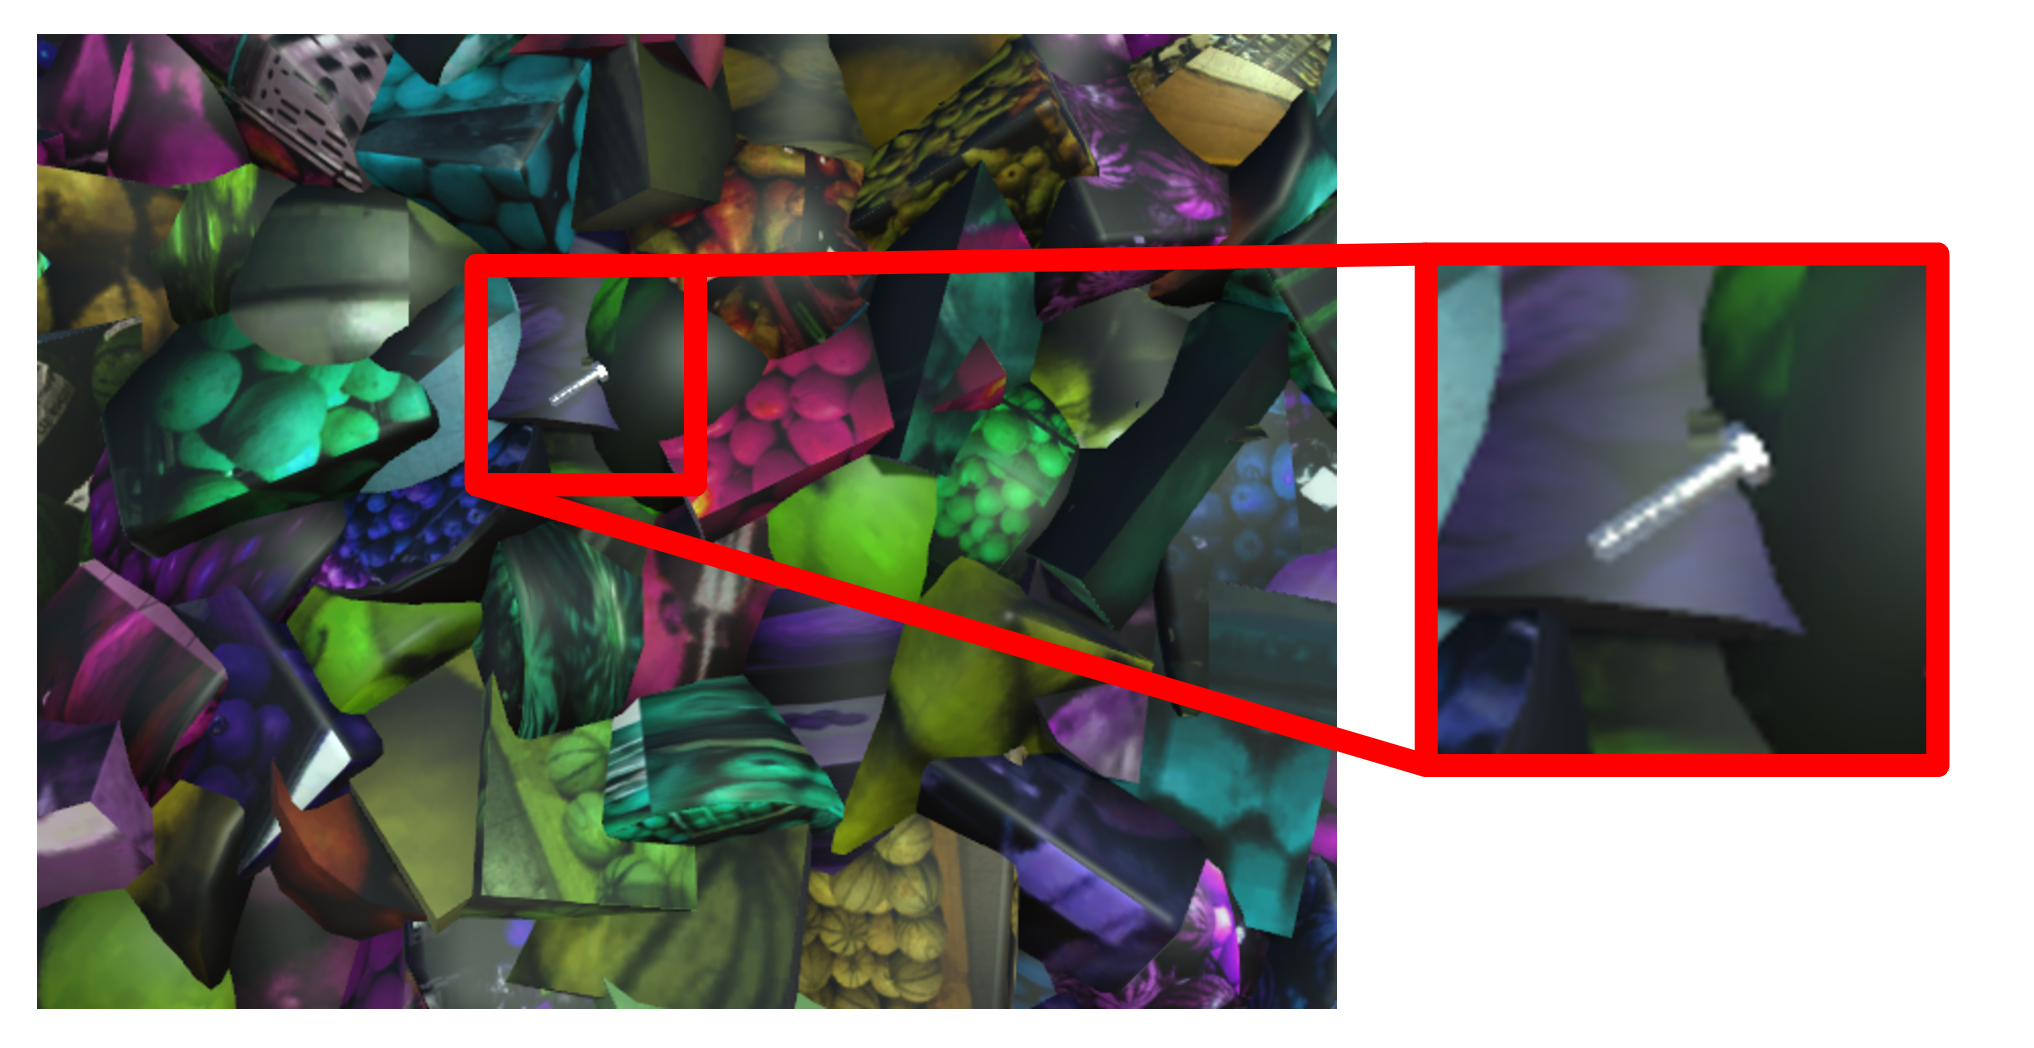
\includegraphics[width=0.6\textwidth]{screwdataset/ScrewDataset.png}
    \caption{One of the images generated with Unity's Perception package for training our model, with a zoom-in on the screw.}
    \label{fig:screwdataset}
\end{figure}

For our dataset, we simulated 10'000 iterations lasting one frame each. We used a model of the M6x30 screw obtained from the FreeCAD Fasteners workbench\cite{Fasteners}, and then used a custom randomizer to set its position and rotation for each iteration. We then used default randomizers provided as samples by Unity as part of its Perception package to generate a background, composed by random 3D shapes placed with random positions, orientations and textures. Finally, we used a custom randomizer to set the lighting color, intensity and origin. A sample image from this dataset appears in figure \ref{fig:screwdataset}.

We can then interface the output of this procedure with EfficientPose using a conversion script, which performs the necessary tasks to make the dataset compatible with the generators used by the network. In this manner we can quickly and easily generate arbitrarily large datasets for training, by first running the Unity scenario, and then running the conversion script for EfficientPose.

\subsection{Training Adjustments}

The original version of EfficientPose is trained on LINEMOD. However, the specifics of LINEMOD and of our own dataset are completely different: LINEMOD has around 1200 images per object, and only about 200 of these are used for training, while ScrewDataset has exactly 10000 images, 9000 of which are used for training and the rest for evaluation. This means that we have to tweak the training parameters to our own dataset.

First, we reduced the number of epochs from 5000 to 100. Since our dataset contains 45 times more images, these two values represent a similar training time for the two different datasets. EfficientPose also by default evaluates the model only every 10 epochs due to the small epoch size; we change this value to evaluate at the end of every epoch.

EfficientPose implements Keras' ReduceLRonPlateau callback to dynamically set the learning rate during training. This is standard practice: large learning rates quickly adjust the model but can lead to fluctuations, local minima and divergence; smaller learning rates avoid these issue but take an excessive amount of time to improve\cite{ReduceLR} the model. This method instead starts with a large learning rate, and then automatically reduces the learning rate whenever training stagnates, thus maintaining a value closer to the ideal By default, EfficientPose halves the LR every time the accuracy does not improve for 25 epochs; we changed this to an 80\% reduction every 5 epochs, to account for the increased number of samples per epoch. The beneficial results of this process are visible in figure \ref{fig:screwdataset_training}, where after epoch 27 a reduction in learning rate causes a sudden drop in training and evaluation loss.

Finally, EfficientPose is concieved to be trained in a single sitting: interrupting and restarting training does not maintain the learning rate, optimizer state and momentum, leading to a rise in training loss before it starts diminishing again after a few epochs. Since we do not want to train the model consecutively for days on end, we implemented custom callbacks that save the optimizer state and learning rate, thus introducing the possibility of interrupting and resuming training if necessary.

\subsection{Results}

\begin{figure}[ht]
    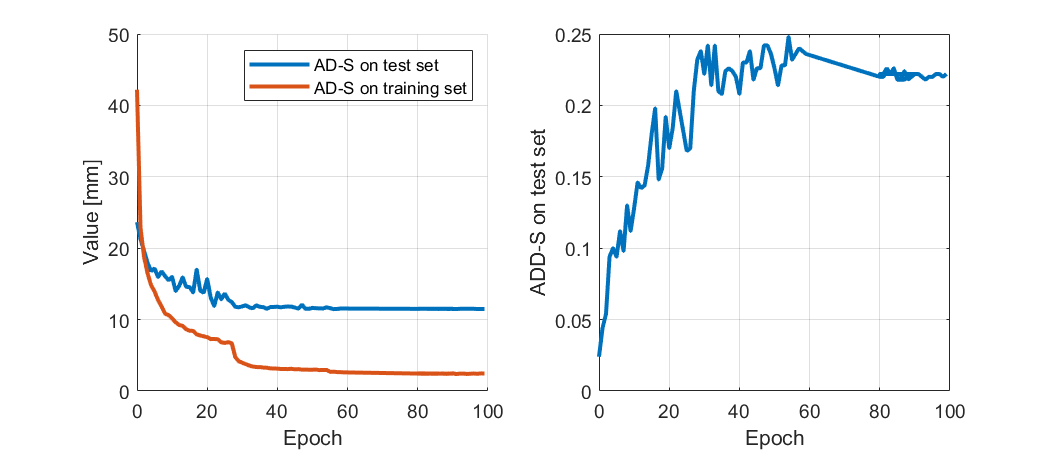
\includegraphics[width=\textwidth]{screwdataset_training.png}
    \caption{Evolution of the loss, AD-S and ADD-S metrics during training. Loss is computed as the AD-S metric on the training dataset.}
    \label{fig:screwdataset_training}
\end{figure}

After 100 epochs of training, the progress of which is shown in figure \ref{fig:screwdataset_training}, the model has a final ADD of 22.2\%, with a peak value obtained during training of 24.8\%, much lower than the 97.35\% reported on LINEMOD. We can hypothesize that the reason for this performance gap is that the rendered dataset is much more difficult than LINEMOD, since we are dealing with a very small, symmetric object hidden inside a chaotic, colorful background with widely different light conditions.

Another serious issue, that is more difficult to convey on paper, is that the model is not able to bridge the reality gap: while testing in real-life scenarios, it failed to identify the screw in most conditions, let alone produce accurate estimations. This means that it generalises poorly outside of the simulated environment, making it essentially unuseable.

\section{Partially Rendered Datasets}

We find ourselves in the situation where our previously trained model has very poor performance. Since EfficientPose works perfectly well with LINEMOD, we can reasonably affirm that the cause for this lies with the training dataset. We can hypothesize two reasons that make this dataset inadequate:

\begin{enumerate}
    \item The training images are too difficult compared to the task we want to perform, preventing the network from learning properly.
    \item The simulated setting for the training images is too different from the setting of the real-life task, thus the model is not able to bridge the reality gap.
\end{enumerate}

We could combat these issues by generating a set of training images that more accurately reflect the task at hand instead of being as general as possible. To do this, we considered two options: re-creating the testing environment in Unity and rendering it together with the object, or using a picture of the enviroment as the background of the rendered image. Between these two, the second is both simpler and faster, and gives more realistic results. Furthermore, changes in the environment can be adapted to by simply taking a new set of pictures.

\subsection{Realistic Placement of Models in Images}

Previous approaches have already generated synthetic data for training by rendering objects on top of photographs. For example, \cite{DPOD} places models from LINEMOD with random poses in front of images from the COCO dataset to achieve this. However, this approach loses information, as while it completely decorrelates the object pose from the environment, in a real-life situation this is often not the case. For example, an object placed on a horizontal surface loses three degrees of freedom, making pose estimation easier in theory. Thus if we wish to generate training images that better reflect the task, we should use pictures of the task area as backgrounds, and then place the 3D models of the dataset objects realistically as they would be seen in real life.

Since our task is the identification and pose estimation of a set of objects placed on a table, we captured a video of the testing table, which had been prepared with an ArUco marker in its centre. After eliminating blurry and off-center frames, we undistorted the images to obtain our final set of backgrounds. Undistorting is an important step for two reasons: primarily it strengthens the correspondence between the virtual sensor with no distortion and the real camera, and secondly training the model on undistorted 3D models rendered on top of distorted images may have resulted in inaccurate predicitons, especially in peripheral areas of the image where the effect is more pronounced. This also means that the images captured during inferencing must also be undistorted, but libraries such as OpenCV make this a trivial task.

Once we have a set of background images, we must then place the dataset object models on the "surface" highlighted by the ArUco marker. We can easily obtain the position and rotation of this surface, as previously described in section \ref*{s:notlearningbasedmethods}. This results in a reference system corresponding to the surface marker, determined using a translation vector $t_s$ and a rotation matrix $R_s$ expressed relative to the camera reference system.

We then want to place the object's model with a random position and orientation on this surface. To do this, we can consider its pose relative to the marker reference system, which is given by a translation vector $t_r$ and a rotation matrix $R_r$. We can select values of $t_r$ and $\text{R}_r$ considering that the condition of "being placed on a surface" imposes three constraints: one on the height and two on the rotation. Mathematically expressed:

\begin{equation*}
    t_r = 
    \begin{bmatrix}
        x_r\\y_r\\0
    \end{bmatrix}
    ,\; \; \text{R}_r =
    \begin{bmatrix}
        \cos \theta_r & - \sin \theta_r & 0 \\
        \sin \theta_r & cos \theta_r & 0 \\
        0 & 0 & 1
    \end{bmatrix}
\end{equation*}

... where $x_r$, $y_r$, and  $\theta_r$ are our three remaining free variables. We can extract their values from pre-defined probability distributions; in our case we used three uniform distributions $U(x_{min}$, $x_{max})$, $U(y_{min}, y_{max})$, and $U(\theta_{min}, \theta_{max})$. The pose $(t, R)$ of the object in the camera reference is then computed as:

\begin{align}
    t &= t_s + \text{R}_s t_r \label{eq:wrongpostionequation} \\
    \text{R} &= \text{R}_s \text{R}_r \nonumber
\end{align}

However, this operation alone is flawed, as it would place the origin of the 3D model on the surface, but for the objects in our dataset, the model origin is in the centre of the object. Therefore we must implement a final roto-translation that places the object on the surface starting from the position computed from \ref*{eq:wrongpostionequation}. This transformation differs based on the object, for example, if we consider the M6x30 screw, this correction transformation $(t_c, \text{R}_c)$ is given by a translation $z_c$ along the z-axis and a rotation by $\theta_c$ around the y-axis:

\begin{equation*}
    t_c = 
    \begin{bmatrix}
        0\\0\\z_c
    \end{bmatrix}
    ,\; \; \text{R}_c =
    \begin{bmatrix}
        \cos \theta_c & 0 & -\sin \theta_c\\
        0 & 1 & 0\\
        \sin \theta_c & 0 &  \cos \theta_c
    \end{bmatrix}
\end{equation*}

...where $z_c$ and $\theta_c$ depend on the dimensions of the screw as follows:

\begin{align*}
    \theta_c &= \frac{\pi}{2} - \arctan \frac{l_2}{l_1}\\
    z_c &= \frac{1}{2}d \sin \theta_c + \frac{1}{2} l \cos \theta_c
\end{align*}

The final pose in camera reference is then given by:

\begin{align*}
    t &= t_s + \text{R}_s t_r + \text{R}_s \text{R}_r t_c\\
    \text{R} &= \text{R}_s \text{R}_r \text{R}_c
\end{align*}

One thing to note is that if an object can have multiple positions on the surface, we consequently have multiple correction transformations to choose from. For example, the M6x30 screw could be on its side or on its head, which implies a choice between two sets of $t_c$, $R_c$.

\subsection{Implementation and Training}

\subsection{Results}

\section{Semantics Applications}